\textsc{\huge Лабораторная работа 16} \\

Используя хвостовую рекурсию, разработать программу, позволяющую найти:
\begin{tasks}
	\task n!,
	\task n-е число Фибоначчи.
\end{tasks}
\begin{lstlisting}
predicates
  Factorial(integer, integer).
  FactorialHelper(integer, integer, integer).

  Fib(integer, integer).
  FibHelper(integer, integer, integer, integer).

clauses
  FactorialHelper(N, Res, Acc) :- N <= 1, Res = Acc, !.
  FactorialHelper(N, Res, Acc) :- UpdAcc = Acc * N, UpdN = N - 1, FactorialHelper(UpdN, Res, UpdAcc).
  Factorial(N, Res) :- FactorialHelper(N, Res, 1).

  FibHelper(N, Res, _, Acc) :- N <= 2, Res = Acc, !.
  FibHelper(N, Res, Prev, Acc) :- UpdN = N - 1, UpdAcc = Prev + Acc, FibHelper(UpdN, Res, Acc, UpdAcc).
  Fib(N, Res) :- FibHelper(N, Res, 1, 1).

goal
  %Factorial(3, Ans).
  Fib(3, Ans).
\end{lstlisting}

\begin{sidewaystable}
	\medskip
	\resizebox{\linewidth}{!}{%
		\tabcolsep=2pt
			\begin{tabular}{|rlll|}
				\begin{tabular}{|rlll|}
					\hline
					\multicolumn{1}{|l|}{\# шага} & \multicolumn{1}{l|}{Состояние резольвенты, и вывод: дальнейшие действия (почему?)} & \multicolumn{1}{l|}{Для каких термов запускается алгоритм унификации: Т1=Т2 и каков результат (и подстановка)} & Дальнейшие действия: прямой ход или откат (к чему приводит?) \\ \hline
					\multicolumn{1}{|r|}{1} & \multicolumn{1}{l|}{\begin{tabular}[c]{@{}l@{}}Factorial(3, Ans)\\ \\ Резольвента не пустая, попытка унификации \\ для подцели, извлекаемой из стека\end{tabular}} & \multicolumn{1}{l|}{\begin{tabular}[c]{@{}l@{}}Factorial(3, Ans), FactorialHelper(N, Res, Acc)\\ \\ Унификация неуспешна (несовпадение функторов)\end{tabular}} & Откат, переход к следующему предложению \\ \hline
					\multicolumn{4}{|l|}{...} \\ \hline
					\multicolumn{1}{|r|}{3} & \multicolumn{1}{l|}{\begin{tabular}[c]{@{}l@{}}Factorial(3, Ans)\\ \\ Резольвента не пустая, попытка унификации \\ для подцели, извлекаемой из стека\end{tabular}} & \multicolumn{1}{l|}{\begin{tabular}[c]{@{}l@{}}Factorial(3, Ans), Factorial(N, Res)\\ \\ Унификация успешна: подстановка\\ \{N = 3, Res = Ans\}\end{tabular}} & Прямой ход, новое состояние резольвенты \\ \hline
					\multicolumn{1}{|r|}{4} & \multicolumn{1}{l|}{\begin{tabular}[c]{@{}l@{}}FactorialHelper(3, Ans, 1).\\ \\ Резольвента не пустая, попытка унификации \\ для подцели, извлекаемой из стека\end{tabular}} & \multicolumn{1}{l|}{\begin{tabular}[c]{@{}l@{}}FactorialHelper(3, Ans, 1), FactorialHelper(N, Res, Acc)\\ \\ Унификация успешна: подстановка\\ \{N = 3, Res = Ans, Acc = 1\}\end{tabular}} & Прямой ход, новое состояние резольвенты \\ \hline
					\multicolumn{1}{|r|}{5} & \multicolumn{1}{l|}{\begin{tabular}[c]{@{}l@{}}3 \textless{}= 1\\ Res = 1\\ !\\ \\ Резольвента не пустая, попытка унификации \\ для подцели, извлекаемой из стека\end{tabular}} & \multicolumn{1}{l|}{3 \textless{}= 1 неверно} & \begin{tabular}[c]{@{}l@{}}Откат к предыдущему состоянию резольвенты\\ \\ Новая подстановка: \{N = 3, Res = Ans\}\end{tabular} \\ \hline
					\multicolumn{1}{|r|}{6} & \multicolumn{1}{l|}{\begin{tabular}[c]{@{}l@{}}FactorialHelper(3, Ans, 1).\\ \\ Резольвента не пустая, попытка унификации \\ для подцели, извлекаемой из стека\end{tabular}} & \multicolumn{1}{l|}{\begin{tabular}[c]{@{}l@{}}FactorialHelper(3, Ans, 1), FactorialHelper(N, Res, Acc)\\ \\ Унификация успешна: подстановка\\ \{N = 3, Res = Ans, Acc = 1\}\end{tabular}} & Прямой ход, новое состояние резольвенты \\ \hline
					\multicolumn{1}{|r|}{7} & \multicolumn{1}{l|}{\begin{tabular}[c]{@{}l@{}}UpdAcc = 1 * 3, \\ UpdN = 3 - 1,\\ FactorialHelper(UpdN, Ans, UpdAcc).\\ \\ \\ Резольвента не пустая, попытка унификации \\ для подцели, извлекаемой из стека\end{tabular}} & \multicolumn{1}{l|}{\begin{tabular}[c]{@{}l@{}}Унификация:\\ UpdAcc = 1 * 3\\ \\ Успешно, подстановка: \{UpdAcc = 3\}\end{tabular}} & Прямой ход, новое состояние резольвенты \\ \hline
					\multicolumn{1}{|r|}{8} & \multicolumn{1}{l|}{\begin{tabular}[c]{@{}l@{}}UpdN = 3 - 1,\\ FactorialHelper(UpdN, Ans, UpdAcc).\\ \\ \\ Резольвента не пустая, попытка унификации \\ для подцели, извлекаемой из стека\end{tabular}} & \multicolumn{1}{l|}{\begin{tabular}[c]{@{}l@{}}Унификация:\\ UpdN = 3 - 1\\ \\ Успешно, подстановка: \{UpdN = 2\}\end{tabular}} & Прямой ход, новое состояние резольвенты \\ \hline
					\multicolumn{1}{|r|}{9} & \multicolumn{1}{l|}{\begin{tabular}[c]{@{}l@{}}FactorialHelper(UpdN, Ans, UpdAcc).\\ \\ \\ Резольвента не пустая, попытка унификации \\ для подцели, извлекаемой из стека\end{tabular}} & \multicolumn{1}{l|}{\begin{tabular}[c]{@{}l@{}}FactorialHelper(2, Ans, 3), FactorialHelper(N, Res, Acc).\\ \\ \\ Унификация успешна, \\ подстановка: \{N = 2, Res = Ans, Acc = 3\}\end{tabular}} & Прямой ход, новое состояние резольвенты \\ \hline
					\multicolumn{1}{|r|}{10} & \multicolumn{1}{l|}{\begin{tabular}[c]{@{}l@{}}2 \textless{}= 1\\ Res = 3\\ !\\ \\ Резольвента не пустая, попытка унификации \\ для подцели, извлекаемой из стека\end{tabular}} & \multicolumn{1}{l|}{2 \textless{}= 1 неверно} & \begin{tabular}[c]{@{}l@{}}Откат к предыдущему состоянию резольвенты\\ \\ Новая подстановка: \{N = 2, Res = Ans, Acc = 3\}\end{tabular} \\ \hline
					\multicolumn{1}{|r|}{11} & \multicolumn{1}{l|}{\begin{tabular}[c]{@{}l@{}}FactorialHelper(2, Ans, 3).\\ \\ \\ Резольвента не пустая, попытка унификации \\ для подцели, извлекаемой из стека"\end{tabular}} & \multicolumn{1}{l|}{\begin{tabular}[c]{@{}l@{}}FactorialHelper(2, Ans, 3), FactorialHelper(N, Res, Acc).\\ \\ \\ Унификация успешна, \\ подстановка: \{N = 2, Res = Ans, Acc = 3\}\end{tabular}} & Прямой ход, новое состояние резольвенты \\ \hline
					\multicolumn{1}{|r|}{12} & \multicolumn{1}{l|}{\begin{tabular}[c]{@{}l@{}}UpdAcc = 3 * 2, \\ UpdN = 2 - 1,\\ FactorialHelper(UpdN, Ans, UpdAcc).\\ \\ \\ Резольвента не пустая, попытка унификации \\ для подцели, извлекаемой из стека\end{tabular}} & \multicolumn{1}{l|}{\begin{tabular}[c]{@{}l@{}}Унификация:\\ UpdAcc = 3 * 2\\ \\ Успешно, подстановка: \{UpdAcc = 6\}\end{tabular}} & Прямой ход, новое состояние резольвенты \\ \hline
					\multicolumn{1}{|r|}{13} & \multicolumn{1}{l|}{\begin{tabular}[c]{@{}l@{}}UpdN = 2 - 1,\\ FactorialHelper(UpdN, Ans, 6).\\ \\ \\ Резольвента не пустая, попытка унификации \\ для подцели, извлекаемой из стека\end{tabular}} & \multicolumn{1}{l|}{\begin{tabular}[c]{@{}l@{}}Унификация:\\ UpdN = 2 - 1\\ \\ Успешно, подстановка: \{UpdN = 1\}\end{tabular}} & Прямой ход, новое состояние резольвенты \\ \hline
				\end{tabular}
			\end{tabular}
	}
\end{sidewaystable}


\begin{sidewaystable}
	\medskip
	\resizebox{\linewidth}{!}{%
		\tabcolsep=2pt
			\begin{tabular}{|rlll|}
				\hline
				\multicolumn{1}{|l|}{\# шага} & \multicolumn{1}{l|}{Состояние резольвенты, и вывод: дальнейшие действия (почему?)} & \multicolumn{1}{l|}{Для каких термов запускается алгоритм унификации: Т1=Т2 и каков результат (и подстановка)} & Дальнейшие действия: прямой ход или откат (к чему приводит?) \\ \hline
				\multicolumn{1}{|r|}{15} & \multicolumn{1}{l|}{\begin{tabular}[c]{@{}l@{}}1 \textless{}= 1\\ Res = 6\\ !\\ \\ Резольвента не пустая, попытка унификации \\ для подцели, извлекаемой из стека\end{tabular}} & \multicolumn{1}{l|}{1 \textless{}= 1 верно} & Прямой ход, новое состояние резольвенты \\ \hline
				\multicolumn{1}{|r|}{16} & \multicolumn{1}{l|}{\begin{tabular}[c]{@{}l@{}}Res = 6\\ !\\ \\ Резольвента не пустая, попытка унификации \\ для подцели, извлекаемой из стека\end{tabular}} & \multicolumn{1}{l|}{\begin{tabular}[c]{@{}l@{}}Унификация:\\ Ans = 6\\ \\ Успешно, подстановка: \{Ans = 6\}\end{tabular}} & Прямой ход, новое состояние резольвенты \\ \hline
				\multicolumn{1}{|r|}{17} & \multicolumn{1}{l|}{\begin{tabular}[c]{@{}l@{}}!\\ \\ Резольвента не пустая, попытка унификации \\ для подцели, извлекаемой из стека\end{tabular}} & \multicolumn{1}{l|}{Встречен системный предикат отсечения} & \begin{tabular}[c]{@{}l@{}}Резольвента пуста.\\ \\ Вывод: Ans = 6\\ \\ Откат с отсечением остаточных предложений процедуры относительно шага 14\\ \\ Новая подстановка: \{N = 2, Res = Ans, Acc = 3\}\end{tabular} \\ \hline
				\multicolumn{1}{|r|}{18} & \multicolumn{1}{l|}{\begin{tabular}[c]{@{}l@{}}FactorialHelper(1, Ans, 6).\\ \\ Резольвента не пустая, попытка унификации \\ для подцели, извлекаемой из стека\end{tabular}} & \multicolumn{1}{l|}{\begin{tabular}[c]{@{}l@{}}FactorialHelper(1, Ans, 6), \\ Factorial(N, Res)\\ \\ Унификация неуспешна(несовпадение функторов)\end{tabular}} & Откат, переход к следующему предложению \\ \hline
				\multicolumn{4}{|l|}{...} \\ \hline
				\multicolumn{1}{|r|}{21} & \multicolumn{1}{l|}{\begin{tabular}[c]{@{}l@{}}FactorialHelper(1, Ans, 6).\\ \\ Резольвента не пустая, попытка унификации \\ для подцели, извлекаемой из стека\end{tabular}} & \multicolumn{1}{l|}{\begin{tabular}[c]{@{}l@{}}FactorialHelper(1, Ans, 6), \\ Fib(N, Res)\\ \\ Унификация неуспешна(несовпадение функторов)\end{tabular}} & \begin{tabular}[c]{@{}l@{}}Конец БЗ достигнут. Откат, переход к следующему предложению\\  относительно пункта 11\\ Новая подстановка: \{N = 2, Res = Ans,  Acc = 1\}\end{tabular} \\ \hline
				\multicolumn{1}{|r|}{22} & \multicolumn{1}{l|}{\begin{tabular}[c]{@{}l@{}}FactorialHelper(2, Ans, 1).\\ \\ \\ Резольвента не пустая, попытка унификации \\ для подцели, извлекаемой из стека"\end{tabular}} & \multicolumn{1}{l|}{\begin{tabular}[c]{@{}l@{}}FactorialHelper(2, Ans, 3), Factorial(N, Acc)\\ Унификация неуспешна(несовпадение функторов)\end{tabular}} & Откат, переход к следующему предложению \\ \hline
				\multicolumn{4}{|l|}{...} \\ \hline
				\multicolumn{1}{|r|}{25} & \multicolumn{1}{l|}{\begin{tabular}[c]{@{}l@{}}FactorialHelper(2, Ans, 1).\\ \\ \\ Резольвента не пустая, попытка унификации \\ для подцели, извлекаемой из стека"\end{tabular}} & \multicolumn{1}{l|}{\begin{tabular}[c]{@{}l@{}}FactorialHelper(2, Ans, 3), \\ Fib(N, Res)\\ \\ Унификация неуспешна(несовпадение функторов)\end{tabular}} & \begin{tabular}[c]{@{}l@{}}Конец БЗ достигнут. Откат, переход к следующему предложению\\  относительно пункта 11\\ Новая подстановка: \{N = 3, Res = Ans,  Acc = 1\}\end{tabular} \\ \hline
				\multicolumn{1}{|r|}{26} & \multicolumn{1}{l|}{\begin{tabular}[c]{@{}l@{}}FactorialHelper(3, Ans, 1).\\ \\ \\ Резольвента не пустая, попытка унификации \\ для подцели, извлекаемой из стека"\end{tabular}} & \multicolumn{1}{l|}{\begin{tabular}[c]{@{}l@{}}FactorialHelper(3, Ans, 1).\\ Factorial(N, Res)\\ \\ Унификация неуспешна (несовпадение функторов)\end{tabular}} & Откат, переход к следующему предложению \\ \hline
				\multicolumn{4}{|l|}{...} \\ \hline
				\multicolumn{1}{|r|}{29} & \multicolumn{1}{l|}{\begin{tabular}[c]{@{}l@{}}FactorialHelper(3, Ans, 1).\\ \\ \\ Резольвента не пустая, попытка унификации \\ для подцели, извлекаемой из стека"\end{tabular}} & \multicolumn{1}{l|}{\begin{tabular}[c]{@{}l@{}}FactorialHelper(3, Ans, 1), \\ Fib(N, Res)\\ \\ Унификация неуспешна(несовпадение функторов)\end{tabular}} & \begin{tabular}[c]{@{}l@{}}Конец БЗ достигнут. Откат, переход к следующему предложению\\  относительно пункта 3\end{tabular} \\ \hline
				\multicolumn{1}{|r|}{30} & \multicolumn{1}{l|}{\begin{tabular}[c]{@{}l@{}}Factorial(3, Ans)\\ \\ Резольвента не пустая, попытка унификации \\ для подцели, извлекаемой из стека\end{tabular}} & \multicolumn{1}{l|}{\begin{tabular}[c]{@{}l@{}}Factorial(3, Ans)\\ FibHelper(N, Res, \_, Acc)\\ \\ Унификация неуспешна(несовпадение функторов)\end{tabular}} & Откат, переход к следующему предложению \\ \hline
				\multicolumn{4}{|l|}{...} \\ \hline
				\multicolumn{1}{|r|}{32} & \multicolumn{1}{l|}{\begin{tabular}[c]{@{}l@{}}Factorial(3, Ans)\\ \\ Резольвента не пустая, попытка унификации \\ для подцели, извлекаемой из стека\end{tabular}} & \multicolumn{1}{l|}{\begin{tabular}[c]{@{}l@{}}Factorial(3, Ans)\\ Fib(N, Res)\\ \\ Унификация неуспешна(несовпадение функторов)\end{tabular}} & Конец БЗ достигнут. Вывод результата \\ \hline
			\end{tabular}
	}
\end{sidewaystable}

\begin{sidewaystable}
	\medskip
	\resizebox{\linewidth}{!}{%
		\tabcolsep=2pt
		\begin{tabular}{|rlll|}
			\hline
			\multicolumn{1}{|l|}{\# шага} & \multicolumn{1}{l|}{Состояние резольвенты, и вывод: дальнейшие действия (почему?)} & \multicolumn{1}{l|}{Для каких термов запускается алгоритм унификации: Т1=Т2 и каков результат (и подстановка)} & Дальнейшие действия: прямой ход или откат (к чему приводит?) \\ \hline
			\multicolumn{1}{|r|}{1} & \multicolumn{1}{l|}{\begin{tabular}[c]{@{}l@{}}Fib(3, Ans).\\ \\ \\ Резольвента не пустая, попытка унификации \\ для подцели, извлекаемой из стека\end{tabular}} & \multicolumn{1}{l|}{\begin{tabular}[c]{@{}l@{}}Fib(3, Ans).\\ FactorialHelper(N, Res, Acc)\\ \\ \\ Унификация неуспешна (несовпадение функторов)\end{tabular}} & Откат, переход к следующему предложению \\ \hline
			\multicolumn{4}{|l|}{...} \\ \hline
			\multicolumn{1}{|r|}{6} & \multicolumn{1}{l|}{\begin{tabular}[c]{@{}l@{}}Fib(3, Ans).\\ \\ \\ Резольвента не пустая, попытка унификации \\ для подцели, извлекаемой из стека\end{tabular}} & \multicolumn{1}{l|}{\begin{tabular}[c]{@{}l@{}}Fib(3, Ans).\\ Fib(N, Res)\\ \\ \\ Унификация успешна: \\ подстановка: \{N = 3, Res = Ans\}\end{tabular}} & Прямой ход, новое состояние резольвенты \\ \hline
			\multicolumn{1}{|r|}{7} & \multicolumn{1}{l|}{\begin{tabular}[c]{@{}l@{}}FibHelper(3, Res, 1, 1).\\ \\ \\ Резольвента не пустая, попытка унификации \\ для подцели, извлекаемой из стека\end{tabular}} & \multicolumn{1}{l|}{\begin{tabular}[c]{@{}l@{}}FibHelper(3, Res, 1, 1).\\ FactorialHelper(N, Res, Acc)\\ \\ Унификация неуспешна (несовпадение функторов)\end{tabular}} & Откат, переход к следующему предложению \\ \hline
			\multicolumn{4}{|l|}{...} \\ \hline
			\multicolumn{1}{|r|}{10} & \multicolumn{1}{l|}{\begin{tabular}[c]{@{}l@{}}FibHelper(3, Res, 1, 1).\\ \\ \\ Резольвента не пустая, попытка унификации \\ для подцели, извлекаемой из стека\end{tabular}} & \multicolumn{1}{l|}{\begin{tabular}[c]{@{}l@{}}FibHelper(3, Res, 1, 1).\\ FibHelper(N, Res, \_, Acc)\\ \\ Унификация успешна:\\ подстановка \{N = 3, Res = Ans, Acc = 1\}\end{tabular}} & Прямой ход, новое состояние резольвенты \\ \hline
			\multicolumn{1}{|r|}{11} & \multicolumn{1}{l|}{\begin{tabular}[c]{@{}l@{}}3 \textless{}= 2,\\ Res = 1, \\ !\\ \\ Резольвента не пустая, попытка унификации \\ для подцели, извлекаемой из стека\end{tabular}} & \multicolumn{1}{l|}{3 \textless{}= 2 неверно} & \begin{tabular}[c]{@{}l@{}}Откат к предыдущему состоянию резольвенты\\ \\ Новая подстановка: \{N = 3, Res = Ans\}\end{tabular} \\ \hline
			\multicolumn{1}{|r|}{12} & \multicolumn{1}{l|}{\begin{tabular}[c]{@{}l@{}}FibHelper(3, Res, 1, 1).\\ \\ \\ Резольвента не пустая, попытка унификации \\ для подцели, извлекаемой из стека\end{tabular}} & \multicolumn{1}{l|}{\begin{tabular}[c]{@{}l@{}}FibHelper(3, Res, 1, 1).\\ FibHelper(N, Res, Prev, Acc)\\ \\ Унификация успешна:\\ подстановка \{N = 3, Res = Ans, Prev = 1, Acc = 1\}\end{tabular}} & Прямой ход, новое состояние резольвенты \\ \hline
			\multicolumn{1}{|r|}{13} & \multicolumn{1}{l|}{\begin{tabular}[c]{@{}l@{}}UpdN = 3 - 1, \\ UpdAcc = 1 + 1,\\ FibHelper(UpdN, Ans, 1, UpdAcc)\\ \\ Резольвента не пустая, попытка унификации \\ для подцели, извлекаемой из стека\end{tabular}} & \multicolumn{1}{l|}{\begin{tabular}[c]{@{}l@{}}Унификация:\\ UpdN = 3 - 1\\ \\ Успешно, подстановка: \{UpdN = 2\}\end{tabular}} & Новое состояние резольвенты \\ \hline
			\multicolumn{1}{|r|}{14} & \multicolumn{1}{l|}{\begin{tabular}[c]{@{}l@{}}UpdAcc = 1 + 1,\\ FibHelper(UpdN, Ans, 1, UpdAcc)\\ \\ Резольвента не пустая, попытка унификации \\ для подцели, извлекаемой из стека\end{tabular}} & \multicolumn{1}{l|}{\begin{tabular}[c]{@{}l@{}}Унификация:\\ UpdAcc = 1 + 1\\ \\ Успешно, подстановка: \{UpdAcc = 2\}\end{tabular}} & Новое состояние резольвенты \\ \hline
			\multicolumn{1}{|r|}{15} & \multicolumn{1}{l|}{\begin{tabular}[c]{@{}l@{}}FibHelper(2, Ans, 1, 2)\\ \\ Резольвента не пустая, попытка унификации \\ для подцели, извлекаемой из стека\end{tabular}} & \multicolumn{1}{l|}{\begin{tabular}[c]{@{}l@{}}FibHelper(2, Ans, 1, 2)\\ FactorialHelper(N, Res, Acc)\\ \\ \\ Унификация неуспешна (несовпадение функторов)\end{tabular}} & Откат, переход к следующему предложению \\ \hline
			\multicolumn{4}{|l|}{...} \\ \hline
			\multicolumn{1}{|r|}{18} & \multicolumn{1}{l|}{\begin{tabular}[c]{@{}l@{}}FibHelper(UpdN, Ans, 1, UpdAcc)\\ \\ Резольвента не пустая, попытка унификации \\ для подцели, извлекаемой из стека\end{tabular}} & \multicolumn{1}{l|}{\begin{tabular}[c]{@{}l@{}}FibHelper(2, Ans, 1, 2)\\ FibHelper(N, Res, \_, Acc)\\ \\ \\ Унификация успешна, подстановка\\ \{N = 2, Res = Ans, Acc = 2\}\end{tabular}} & Новое состояние резольвенты \\ \hline
			\multicolumn{1}{|r|}{19} & \multicolumn{1}{l|}{\begin{tabular}[c]{@{}l@{}}2 \textless{}= 2\\ Res = Acc\\ !\\ \\ Резольвента не пустая, попытка унификации \\ для подцели, извлекаемой из стека\end{tabular}} & \multicolumn{1}{l|}{2 \textless{}= 2 верно} & Новое состояние резольвенты \\ \hline
		\end{tabular}
	}
\end{sidewaystable}

\begin{sidewaystable}
	\medskip
	\resizebox{\linewidth}{!}{%
		\tabcolsep=2pt
		\begin{tabular}{|rlll|}
			\hline
			\multicolumn{1}{|l|}{\# шага} & \multicolumn{1}{l|}{Состояние резольвенты, и вывод: дальнейшие действия (почему?)} & \multicolumn{1}{l|}{Для каких термов запускается алгоритм унификации: Т1=Т2 и каков результат (и подстановка)} & Дальнейшие действия: прямой ход или откат (к чему приводит?) \\ \hline
			\multicolumn{1}{|r|}{20} & \multicolumn{1}{l|}{\begin{tabular}[c]{@{}l@{}}Res = 2\\ !\\ \\ Резольвента не пустая, попытка унификации \\ для подцели, извлекаемой из стека\end{tabular}} & \multicolumn{1}{l|}{\begin{tabular}[c]{@{}l@{}}Унификация:\\ Res = 2\\ \\ Успешно, подстановка: \{Res = 2\}\end{tabular}} & Новое состояние резольвенты \\ \hline
			\multicolumn{1}{|r|}{21} & \multicolumn{1}{l|}{\begin{tabular}[c]{@{}l@{}}!\\ \\ Резольвента не пустая, попытка унификации \\ для подцели, извлекаемой из стека\end{tabular}} & \multicolumn{1}{l|}{Встречен системный предикат отсечения} & \begin{tabular}[c]{@{}l@{}}Резольвента пуста.\\ \\ Вывод: Ans = 2\\ \\ Откат с отсечением остаточных предложений процедуры относительно шага 18\\ \\ Новая подстановка: \{N = 2, Res = Ans\}\end{tabular} \\
			\hline
			\multicolumn{1}{|r|}{22} & \multicolumn{1}{l|}{\begin{tabular}[c]{@{}l@{}}FibHelper(2, Ans, 1, 2)\\ \\ Резольвента не пустая, попытка унификации \\ для подцели, извлекаемой из стека\end{tabular}} & \multicolumn{1}{l|}{\begin{tabular}[c]{@{}l@{}}FibHelper(2, Ans, 1, 2)\\ Fib(N, Res)\\ \\ Унификация неуспешна (несовпадение функторов)\end{tabular}} & \begin{tabular}[c]{@{}l@{}}Конец БЗ достигнут. Откат, переход к следующему предложению\\  относительно пункта 12\\ Новая подстановка: \{N = 3, Res = Ans\}\end{tabular} \\ 
			\hline
			\multicolumn{1}{|r|}{23} & \multicolumn{1}{l|}{\begin{tabular}[c]{@{}l@{}}FibHelper(3, Ans, 1, 1)\\ \\ Резольвента не пустая, попытка унификации \\ для подцели, извлекаемой из стека\end{tabular}} & \multicolumn{1}{l|}{\begin{tabular}[c]{@{}l@{}}FibHelper(3, Ans, 1, 1)\\ Fib(N, Res)\\ \\ Унификация неуспешна (несовпадение функторов)\end{tabular}} & \begin{tabular}[c]{@{}l@{}}Конец БЗ достигнут. Откат, переход к следующему предложению\\  относительно пункта 6\end{tabular} \\ \hline
			\multicolumn{1}{|r|}{24} & \multicolumn{1}{l|}{\begin{tabular}[c]{@{}l@{}}Fib(3, Ans).\\ \\ \\ Резольвента не пустая, попытка унификации \\ для подцели, извлекаемой из стека\end{tabular}} & \multicolumn{1}{l|}{-} & Конец БЗ достигнут. Вывод результата на экран \\ \hline
		\end{tabular}
	}
\end{sidewaystable}

~\newpage
\textsc{\huge Лабораторная работа 17} \\

Используя хвостовую рекурсию, разработать эффективную программу (комментируя назначение аргументов), позволяющую:
\begin{tasks}
	\task Найти длину списка (по верхнему уровню);
	\task Найти сумму элементов числового списка;
	\task Найти сумму элементов числового списка, стоящих на нечетных позициях исходного списка (нумерация от 0);
\end{tasks}

\begin{lstlisting}
domains 
  list = integer*.
predicates
  ListLen(list, integer).
  ListLenHelper(list, integer, integer).

  ListSum(list, integer).
  ListSumHelper(list, integer, integer).

  ListOddSum(list, integer).
  ListOddSumHelper(list, integer, integer).

clauses
  ListLenHelper([], Res, Acc) :- Res = Acc, !.
  ListLenHelper([_|T], Res, Acc) :- UpdAcc = Acc + 1, ListlenHelper(T, Res, UpdAcc).
  ListLen(List, Res) :- ListLenHelper(List, Res, 0).

  ListSumHelper([], Res, Acc) :- Res = Acc, !.
  ListSumHelper([H|T], Res, Acc) :- UpdAcc = Acc + H, ListSumHelper(T, Res, UpdAcc).
  ListSum(List, Res) :- ListSumHelper(List, Res, 0).

  ListOddSumHelper([], Res, Acc) :- Res = Acc, !.
  ListOddSumHelper([H|[_|T]], Res, Acc) :- UpdAcc = Acc + H, ListOddSumHelper(T, Res, UpdAcc), !.
  ListOddSumHelper([H|_], Res, Acc) :- Res = Acc + H.

  ListOddSum(List, Res) :- ListOddSumHelper(List, Res, 0).

goal
  ListSum([3, 4, 5], Res).
\end{lstlisting}

\begin{sidewaystable}
	\medskip
	\resizebox{\linewidth}{!}{%
		\tabcolsep=2pt
			\begin{tabular}{|rlll|}
				\hline
				\multicolumn{1}{|l|}{\# шага} & \multicolumn{1}{l|}{Состояние резольвенты, и вывод: дальнейшие действия (почему?)} & \multicolumn{1}{l|}{Для каких термов запускается алгоритм унификации: Т1=Т2 и каков результат (и подстановка)} & Дальнейшие действия: прямой ход или откат (к чему приводит?) \\ \hline
				\multicolumn{1}{|r|}{1} & \multicolumn{1}{l|}{\begin{tabular}[c]{@{}l@{}}ListSum({[}3, 4, 5{]}, Res).\\ \\ Резольвента не пустая, попытка унификации \\ для подцели, извлекаемой из стека\end{tabular}} & \multicolumn{1}{l|}{\begin{tabular}[c]{@{}l@{}}ListSum({[}3, 4, 5{]}, Res), ListLenHelper({[}{]}, Res, Acc)\\ \\ Унификация неуспешна (несовпадение функторов)\end{tabular}} & Откат, переход к следующему предложению \\ \hline
				\multicolumn{4}{|l|}{...} \\ \hline
				\multicolumn{1}{|r|}{6} & \multicolumn{1}{l|}{\begin{tabular}[c]{@{}l@{}}ListSum({[}3, 4, 5{]}, Res).\\ \\ Резольвента не пустая, попытка унификации \\ для подцели, извлекаемой из стека\end{tabular}} & \multicolumn{1}{l|}{\begin{tabular}[c]{@{}l@{}}ListSum({[}3, 4, 5{]}, Res), ListSum(List, Res)\\ \\ Унификация успешна: подстановка\\ \{List = {[}3, 4, 5{]}, Res = Res, Acc = 0\}\end{tabular}} & Новое состояние резольвенты \\ \hline
				\multicolumn{1}{|r|}{7} & \multicolumn{1}{l|}{\begin{tabular}[c]{@{}l@{}}ListSumHelper({[}3, 4, 5{]}, Res, 0).\\ \\ Резольвента не пустая, попытка унификации \\ для подцели, извлекаемой из стека\end{tabular}} & \multicolumn{1}{l|}{\begin{tabular}[c]{@{}l@{}}ListSumHelper({[}3, 4, 5{]}, Res, 0), \\ ListLenHelper({[}{]}, Res, Acc)\\ \\ Унификация неуспешна (несовпадение функторов)\end{tabular}} & Откат, переход к следующему предложению \\ \hline
				\multicolumn{4}{|l|}{...} \\ \hline
				\multicolumn{1}{|r|}{10} & \multicolumn{1}{l|}{\begin{tabular}[c]{@{}l@{}}ListSumHelper({[}3, 4, 5{]}, Res, 0).\\ \\ Резольвента не пустая, попытка унификации \\ для подцели, извлекаемой из стека\end{tabular}} & \multicolumn{1}{l|}{\begin{tabular}[c]{@{}l@{}}ListSumHelper({[}3, 4, 5{]}, Res, 0), \\ ListSumHelper({[}{]}, Res, Acc)\\ \\ Унификация неуспешна (несовпадение первых аргументов)\end{tabular}} & Откат, переход к следующему предложению \\ \hline
				\multicolumn{1}{|r|}{11} & \multicolumn{1}{l|}{\begin{tabular}[c]{@{}l@{}}ListSumHelper({[}3, 4, 5{]}, Res, 0).\\ \\ Резольвента не пустая, попытка унификации \\ для подцели, извлекаемой из стека\end{tabular}} & \multicolumn{1}{l|}{\begin{tabular}[c]{@{}l@{}}ListSumHelper({[}3, 4, 5{]}, Res, 0), \\ ListSumHelper({[}H|T{]}, Res, Acc)\\ \\ Унификация успешна, подстановка\\ \{H = 1, List = {[}4, 5{]}, Res = Res, Acc = 0\}\end{tabular}} & Новое состояние резольвенты, прямой ход \\ \hline
				\multicolumn{1}{|r|}{12} & \multicolumn{1}{l|}{\begin{tabular}[c]{@{}l@{}}UpdAcc = 0 + 3\\ ListSumHelper({[}4, 5{]}, Res, UpdAcc)\\ \\ Резольвента не пустая, попытка унификации \\ для подцели, извлекаемой из стека\end{tabular}} & \multicolumn{1}{l|}{\begin{tabular}[c]{@{}l@{}}Унификация:\\ UpdAcc = 0 + 3\\ \\ Успешно, подстановка: \{UpdAcc = 3\}\end{tabular}} & Новое состояние резольвенты, прямой ход \\ \hline
				\multicolumn{1}{|r|}{13} & \multicolumn{1}{l|}{\begin{tabular}[c]{@{}l@{}}ListSumHelper({[}4, 5{]}, Res, UpdAcc)\\ \\ Резольвента не пустая, попытка унификации \\ для подцели, извлекаемой из стека\end{tabular}} & \multicolumn{1}{l|}{\begin{tabular}[c]{@{}l@{}}ListSumHelper({[}4, 5{]}, Res, UpdAcc), ListLenHelper({[}{]}, Res, Acc)\\ \\ Унификация неуспешна (несовпадение функторов)\end{tabular}} & Откат, переход к следующему предложению \\ \hline
				\multicolumn{4}{|l|}{...} \\ \hline
				\multicolumn{1}{|r|}{16} & \multicolumn{1}{l|}{\begin{tabular}[c]{@{}l@{}}ListSumHelper({[}4, 5{]}, Res, UpdAcc)\\ \\ Резольвента не пустая, попытка унификации \\ для подцели, извлекаемой из стека\end{tabular}} & \multicolumn{1}{l|}{\begin{tabular}[c]{@{}l@{}}ListSumHelper({[}4, 5{]}, Res, UpdAcc), ListSumHelper({[}H|T{]}, Res, Acc)\\ \\ Унификация успешна, подстановка\\ \{H = 4, List = {[}5{]}, Res = Res, Acc = 3\}\end{tabular}} & Новое состояние резольвенты, прямой ход \\ \hline
				\multicolumn{1}{|r|}{17} & \multicolumn{1}{l|}{\begin{tabular}[c]{@{}l@{}}UpdAcc = 3 + 4\\ ListSumHelper({[}5{]}, Res, UpdAcc)\\ \\ Резольвента не пустая, попытка унификации \\ для подцели, извлекаемой из стека\end{tabular}} & \multicolumn{1}{l|}{\begin{tabular}[c]{@{}l@{}}Унификация:\\ UpdAcc = 3 + 4\\ \\ Успешно, подстановка: \{UpdAcc = 7\}\end{tabular}} & Новое состояние резольвенты, прямой ход \\ \hline
				\multicolumn{1}{|r|}{18} & \multicolumn{1}{l|}{\begin{tabular}[c]{@{}l@{}}ListSumHelper({[}5{]}, Res, 7).\\ \\ Резольвента не пустая, попытка унификации \\ для подцели, извлекаемой из стека\end{tabular}} & \multicolumn{1}{l|}{\begin{tabular}[c]{@{}l@{}}ListSumHelper({[}5{]}, Res, 7), ListLenHelper({[}{]}, Res, Acc)\\ \\ Унификация неуспешна (несовпадение функторов)\end{tabular}} & Откат, переход к следующему предложению \\ \hline
				\multicolumn{4}{|l|}{...} \\ \hline
				\multicolumn{1}{|r|}{22} & \multicolumn{1}{l|}{\begin{tabular}[c]{@{}l@{}}ListSumHelper({[}5{]}, Res, 7)\\ \\ Резольвента не пустая, попытка унификации \\ для подцели, извлекаемой из стека\end{tabular}} & \multicolumn{1}{l|}{\begin{tabular}[c]{@{}l@{}}ListSumHelper({[}5{]}, Res, 7), ListSumHelper({[}H|T{]}, Res, Acc)\\ \\ Унификация успешна, подстановка\\ \{H = 5, List = {[}{]}, Res = Res, Acc = 7\}\end{tabular}} & Новое состояние резольвенты, прямой ход \\ \hline
				\multicolumn{1}{|r|}{23} & \multicolumn{1}{l|}{\begin{tabular}[c]{@{}l@{}}UpdAcc = 7 + 5\\ ListSumHelper({[}{]}, Res, UpdAcc)\\ \\ Резольвента не пустая, попытка унификации \\ для подцели, извлекаемой из стека\end{tabular}} & \multicolumn{1}{l|}{\begin{tabular}[c]{@{}l@{}}Унификация:\\ UpdAcc = 7 + 5\\ \\ Успешно, подстановка: \{UpdAcc = 12\}\end{tabular}} & Новое состояние резольвенты, прямой ход \\ \hline
				\multicolumn{1}{|r|}{24} & \multicolumn{1}{l|}{\begin{tabular}[c]{@{}l@{}}ListSumHelper({[}{]}, Res, 12).\\ \\ Резольвента не пустая, попытка унификации \\ для подцели, извлекаемой из стека\end{tabular}} & \multicolumn{1}{l|}{\begin{tabular}[c]{@{}l@{}}ListSumHelper({[}{]}, Res, 12), \\ ListLenHelper({[}{]}, Res, Acc)\\ \\ Унификация неуспешна (несовпадение функторов)\end{tabular}} & Откат, переход к следующему предложению \\ \hline
				\multicolumn{4}{|l|}{...} \\ \hline
			\end{tabular}
	}
\end{sidewaystable}
%
\begin{sidewaystable}
	\medskip
	\resizebox{\linewidth}{!}{%
		\tabcolsep=2pt
		\begin{tabular}{|rlll|}
			\hline
			\multicolumn{1}{|l|}{\# шага} & \multicolumn{1}{l|}{Состояние резольвенты, и вывод: дальнейшие действия (почему?)} & \multicolumn{1}{l|}{Для каких термов запускается алгоритм унификации: Т1=Т2 и каков результат (и подстановка)} & Дальнейшие действия: прямой ход или откат (к чему приводит?) \\ \hline
			\multicolumn{1}{|r|}{27} & \multicolumn{1}{l|}{\begin{tabular}[c]{@{}l@{}}ListSumHelper({[}{]}, Res, 12)\\ \\ Резольвента не пустая, попытка унификации \\ для подцели, извлекаемой из стека\end{tabular}} & \multicolumn{1}{l|}{\begin{tabular}[c]{@{}l@{}}ListSumHelper({[}{]}, Res, UpdAcc), ListSumHelper({[}{]}, Res, Acc)\\ \\ Унификация успешна, подстановка\\ \{Res = Res, Acc = 12\}\end{tabular}} & Новое состояние резольвенты, прямой ход \\ \hline
			\multicolumn{1}{|r|}{28} & \multicolumn{1}{l|}{\begin{tabular}[c]{@{}l@{}}Res = 12\\ !\\ \\ Резольвента не пустая, попытка унификации \\ для подцели, извлекаемой из стека\end{tabular}} & \multicolumn{1}{l|}{\begin{tabular}[c]{@{}l@{}}Унификация:\\ Res = 12\\ \\ Успешно, подстановка: \{Res = 12\}\end{tabular}} & Новое состояние резольвенты, прямой ход \\ \hline
			\multicolumn{1}{|r|}{29} & \multicolumn{1}{l|}{\begin{tabular}[c]{@{}l@{}}!\\ \\ Резольвента не пустая, попытка унификации \\ для подцели, извлекаемой из стека\end{tabular}} & \multicolumn{1}{l|}{Встречен системный предикат отсечения} & \begin{tabular}[c]{@{}l@{}}Резольвента пуста.\\ \\ Запомнить Res = 12\\ \\ Откат с отсечением остаточных предложений процедуры относительно шага 27\end{tabular} \\ \hline
			\multicolumn{1}{|r|}{30} & \multicolumn{1}{l|}{\begin{tabular}[c]{@{}l@{}}ListSumHelper({[}{]}, Res, 12)\\ \\ Резольвента не пустая, попытка унификации \\ для подцели, извлекаемой из стека\end{tabular}} & \multicolumn{1}{l|}{\begin{tabular}[c]{@{}l@{}}ListSumHelper({[}{]}, Res, 12), ListSumHelper({[}H|T{]}, Res, Acc)\\ \\ Унификация неуспешна (несовпадение первых аргументов)\end{tabular}} & Откат, переход к следующему предложению \\ \hline
			\multicolumn{4}{|l|}{...} \\ \hline
			\multicolumn{1}{|r|}{35} & \multicolumn{1}{l|}{\begin{tabular}[c]{@{}l@{}}ListSumHelper({[}{]}, Res, 12)\\ \\ Резольвента не пустая, попытка унификации \\ для подцели, извлекаемой из стека\end{tabular}} & \multicolumn{1}{l|}{\begin{tabular}[c]{@{}l@{}}ListSumHelper({[}{]}, Res, 12), ListOddSum(List, Res)\\ \\ Унификация неуспешна (несовпадение функторов)\end{tabular}} & \begin{tabular}[c]{@{}l@{}}Конец БЗ достигнут. Откат, переход к следующему предложению\\  относительно пункта 22\\ Новая подстановка: \{List = {[}5{]}, Res=Res, Acc = 7\}\end{tabular} \\ \hline
			\multicolumn{1}{|r|}{36} & \multicolumn{1}{l|}{\begin{tabular}[c]{@{}l@{}}ListSumHelper({[}5{]}, Res, 7)\\ \\ Резольвента не пустая, попытка унификации \\ для подцели, извлекаемой из стека\end{tabular}} & \multicolumn{1}{l|}{\begin{tabular}[c]{@{}l@{}}ListSumHelper({[}5{]}, Res, 7), ListSum(List, Res)\\ \\ Унификация неуспешна (несовпадение функторов)\end{tabular}} & Откат, переход к следующему предложению \\ \hline
			\multicolumn{4}{|l|}{...} \\ \hline
			\multicolumn{1}{|r|}{40} & \multicolumn{1}{l|}{\begin{tabular}[c]{@{}l@{}}ListSumHelper({[}5{]}, Res, 7)\\ \\ Резольвента не пустая, попытка унификации \\ для подцели, извлекаемой из стека\end{tabular}} & \multicolumn{1}{l|}{\begin{tabular}[c]{@{}l@{}}ListSumHelper({[}5{]}, Res, 7), ListOddSum(List, Res)\\ \\ Унификация неуспешна (несовпадение функторов)\end{tabular}} & \begin{tabular}[c]{@{}l@{}}Конец БЗ достигнут. Откат, переход к следующему предложению\\  относительно пункта 16\\ Новая подстановка: \{List = {[}4, 5{]}, Res=Res, Acc = 3\}\end{tabular} \\ \hline
			\multicolumn{1}{|r|}{41} & \multicolumn{1}{l|}{\begin{tabular}[c]{@{}l@{}}ListSumHelper({[}4, 5{]}, Res, 3)\\ \\ Резольвента не пустая, попытка унификации \\ для подцели, извлекаемой из стека\end{tabular}} & \multicolumn{1}{l|}{\begin{tabular}[c]{@{}l@{}}ListSumHelper({[}4, 5{]}, Res, 3), ListSum(List, Res)\\ \\ Унификация неуспешна (несовпадение функторов)\end{tabular}} & Откат, переход к следующему предложению \\ \hline
			\multicolumn{4}{|l|}{...} \\ \hline
			\multicolumn{1}{|r|}{45} & \multicolumn{1}{l|}{\begin{tabular}[c]{@{}l@{}}ListSumHelper({[}4, 5{]}, Res, 3)\\ \\ Резольвента не пустая, попытка унификации \\ для подцели, извлекаемой из стека\end{tabular}} & \multicolumn{1}{l|}{\begin{tabular}[c]{@{}l@{}}ListSumHelper({[}4, 5{]}, Res, 3),ListOddSum(List, Res)\\ \\ Унификация неуспешна (несовпадение функторов)\end{tabular}} & \begin{tabular}[c]{@{}l@{}}Конец БЗ достигнут. Откат, переход к следующему предложению\\  относительно пункта 6\\ Новая подстановка: \{List = {[}3, 4, 5{]}, Res=Res, Acc = 0\}\end{tabular} \\ \hline
			\multicolumn{1}{|r|}{46} & \multicolumn{1}{l|}{\begin{tabular}[c]{@{}l@{}}ListSumHelper({[}3, 4, 5{]}, Res, 0)\\ \\ Резольвента не пустая, попытка унификации \\ для подцели, извлекаемой из стека\end{tabular}} & \multicolumn{1}{l|}{\begin{tabular}[c]{@{}l@{}}ListSumHelper({[}3, 4, 5{]}, Res, 0),ListSum(List, Res)\\ \\ Унификация неуспешна (несовпадение функторов)\end{tabular}} & Откат, переход к следующему предложению \\ \hline
			\multicolumn{4}{|l|}{...} \\ \hline
			\multicolumn{1}{|r|}{50} & \multicolumn{1}{l|}{\begin{tabular}[c]{@{}l@{}}ListSumHelper({[}3, 4, 5{]}, Res, 0)\\ \\ Резольвента не пустая, попытка унификации \\ для подцели, извлекаемой из стека\end{tabular}} & \multicolumn{1}{l|}{\begin{tabular}[c]{@{}l@{}}ListSumHelper({[}3, 4, 5{]}, Res, 0),ListOddSum(List, Res)\\ \\ Унификация неуспешна (несовпадение функторов)\end{tabular}} & Конец БЗ достигнут. Вывод результата на экран \\ \hline
			
		\end{tabular}
		
	}
\end{sidewaystable}

~\newpage
\textsc{\huge Лабораторная работа 18} \\
Используя хвостовую рекурсию, разработать, комментируя аргументы,
эффективную программу, позволяющую:
\begin{tasks}
	\task Сформировать список из элементов числового списка, больших заданного
	значения;
	\task Сформировать список из элементов, стоящих на нечетных позициях исходного списка (нумерация от 0);
	\task Удалить заданный элемент из списка (один или все вхождения);
	\task Преобразовать список в множество (можно использовать ранее разработанные процедуры).
\end{tasks}
\begin{lstlisting}
domains
  list = integer*.
predicates
  Append(list, list, list).
  ListGreaterThen(list, integer, list).
  ListLeaveOdd(list, list).
  ListRemoveElem(list, integer, list).
  ListIncludes(list, integer).
  ListToSet(list, list).
clauses
  Append([_|T], List, [_|Res]) :- Append(T, List, Res), !.
  Append([], List, List).
  ListGreaterThen([H|T], N, [H|Res]) :- H > N, !, ListGreaterThen(T, N, Res), !.
  ListGreaterThen([_|T], N, Res) :- ListGreaterThen(T, N, Res), !.
  ListGreaterThen([], _, []).
  ListLeaveOdd([H|[_|T]], [H|Res]) :- ListLeaveOdd(T, Res), !.
  ListLeaveOdd(List, List).
  ListRemoveElem([H|T], Item, Res) :- Item = H, !, ListRemoveElem(T, Item, Res).
  ListRemoveElem([H|T], Item, [H|Res]) :- ListRemoveElem(T, Item, Res), !.
  ListRemoveElem(List, _, List).
  ListIncludes([_|T], Item) :- ListIncludes(T, Item), !.
  ListIncludes([H|_], H).
  ListToSet([H|T], Res) :- ListIncludes(T, H), !, ListToSet(T, Res).
  ListToSet([H|T], [H|Res]) :- ListToSet(T, Res), !.
  ListToSet(List, List).
goal
  ListGreaterThen([3, 4, 5], 4, List).
\end{lstlisting}

\begin{sidewaystable}
	\medskip
	\resizebox{\linewidth}{!}{%
		\tabcolsep=2pt
				\begin{tabular}{|rlll|l}
					\cline{1-4}
					\multicolumn{1}{|l|}{\# шага} & \multicolumn{1}{l|}{Состояние резольвенты, и вывод: дальнейшие действия (почему?)}                                                                                                                           & \multicolumn{1}{l|}{Для каких термов запускается алгоритм унификации: Т1=Т2 и каков результат (и подстановка)}                                                                                                                                       & Дальнейшие действия: прямой ход или откат (к чему приводит?)                                                                                    &  \\ \cline{1-4}
					\multicolumn{1}{|r|}{1}       & \multicolumn{1}{l|}{\begin{tabular}[c]{@{}l@{}}ListGreaterThen({[}3, 4, 5{]}, 4, List).\\ \\ Резольвента не пустая, попытка унификации \\ для подцели, извлекаемой из стека\end{tabular}}                    & \multicolumn{1}{l|}{\begin{tabular}[c]{@{}l@{}}ListGreaterThen({[}3, 4, 5{]}, 4, List), Append({[}\_|T{]}, List, {[}\_|Res{]})\\ \\ Унификация неуспешна (несовпадение функторов)\end{tabular}}                                                      & Откат, переход к следующему предложению                                                                                                         &  \\ \cline{1-4}
					\multicolumn{4}{|l|}{...}                                                                                                                                                                                                                                                                                                                                                                                                                                                                                                                                                                                                                             &  \\ \cline{1-4}
					\multicolumn{1}{|r|}{3}       & \multicolumn{1}{l|}{\begin{tabular}[c]{@{}l@{}}ListGreaterThen({[}3, 4, 5{]}, 4, List).\\ \\ Резольвента не пустая, попытка унификации \\ для подцели, извлекаемой из стека\end{tabular}}                    & \multicolumn{1}{l|}{\begin{tabular}[c]{@{}l@{}}ListGreaterThen({[}3, 4, 5{]}, 4, List), ListGreaterThen({[}H|T{]}, N, {[}H|Res{]})\\ \\ УНификация успешна, подстановка\\ \{H = {[}3{]},  T = {[}4, 5{]}, N = 4,  {[}H|Res{]} = List\}\end{tabular}} & Новое состояние резольвенты, прямой ход                                                                                                         &  \\ \cline{1-4}
					\multicolumn{1}{|r|}{4}       & \multicolumn{1}{l|}{\begin{tabular}[c]{@{}l@{}}1 \textgreater 4\\ !\\ ListGreaterThen({[}4, 5{]}, 4, List)\\ \\ Резольвента не пустая, попытка унификации \\ для подцели, извлекаемой из стека\end{tabular}} & \multicolumn{1}{l|}{1 \textless 4 неверно}                                                                                                                                                                                                           & Откат, возврат к предыдущему состоянию резольвенты, переход к следующему предложению                                                            &  \\ \cline{1-4}
					\multicolumn{1}{|r|}{5}       & \multicolumn{1}{l|}{\begin{tabular}[c]{@{}l@{}}ListGreaterThen({[}3, 4, 5{]}, 4, List).\\ \\ Резольвента не пустая, попытка унификации \\ для подцели, извлекаемой из стека\end{tabular}}                    & \multicolumn{1}{l|}{\begin{tabular}[c]{@{}l@{}}ListGreaterThen({[}3, 4, 5{]}, 4, List), ListGreaterThen({[}\_|T{]}, N, Res)\\ \\ УНификация успешна, подстановка\\ \{T = {[}4, 5{]}, N = 4,  Res = List\}\end{tabular}}                              & Новое состояние резольвенты, прямой ход                                                                                                         &  \\ \cline{1-4}
					\multicolumn{1}{|r|}{6}       & \multicolumn{1}{l|}{\begin{tabular}[c]{@{}l@{}}ListGreaterThen({[}4, 5{]}, 4, List),\\ !\\ \\ Резольвента не пустая, попытка унификации \\ для подцели, извлекаемой из стека\end{tabular}}                   & \multicolumn{1}{l|}{\begin{tabular}[c]{@{}l@{}}ListGreaterThen({[}4, 5{]}, 4, List), Append({[}\_|T{]}, List, {[}\_|Res{]})\\ \\ Унификация неуспешна (несовпадение функторов)\end{tabular}}                                                         & Откат, переход к следующему предложению                                                                                                         &  \\ \cline{1-4}
					\multicolumn{4}{|l|}{...}                                                                                                                                                                                                                                                                                                                                                                                                                                                                                                                                                                                                                             &  \\ \cline{1-4}
					\multicolumn{1}{|r|}{8}       & \multicolumn{1}{l|}{\begin{tabular}[c]{@{}l@{}}ListGreaterThen({[}4, 5{]}, 4, List),\\ !\\ \\ Резольвента не пустая, попытка унификации \\ для подцели, извлекаемой из стека\end{tabular}}                   & \multicolumn{1}{l|}{\begin{tabular}[c]{@{}l@{}}ListGreaterThen({[}3, 4, 5{]}, 4, List), ListGreaterThen({[}H|T{]}, N, Res)\\ \\ УНификация успешна, подстановка\\ \{H = 4, T = {[}5{]}, N = 4,  Res = List\}\end{tabular}}                           & Новое состояние резольвенты, прямой ход                                                                                                         &  \\ \cline{1-4}
					\multicolumn{1}{|r|}{9}       & \multicolumn{1}{l|}{\begin{tabular}[c]{@{}l@{}}4 \textgreater 4\\ !\\ ListGreaterThen({[}5{]}, 4, List)\\ \\ Резольвента не пустая, попытка унификации \\ для подцели, извлекаемой из стека\end{tabular}}    & \multicolumn{1}{l|}{4 \textless 4 неверно}                                                                                                                                                                                                           & Откат, возврат к предыдущему состоянию резольвенты, переход к следующему предложению                                                            &  \\ \cline{1-4}
					\multicolumn{1}{|r|}{10}      & \multicolumn{1}{l|}{\begin{tabular}[c]{@{}l@{}}ListGreaterThen({[}4, 5{]}, 4, List),\\ !\\ \\ Резольвента не пустая, попытка унификации \\ для подцели, извлекаемой из стека\end{tabular}}                   & \multicolumn{1}{l|}{\begin{tabular}[c]{@{}l@{}}ListGreaterThen({[}4, 5{]}, 4, List), ListGreaterThen({[}\_|T{]}, N, Res)\\ \\ УНификация успешна, подстановка\\ \{T = {[}5{]}, N = 4,  {[}4|Res{]} = List\}\end{tabular}}                            & Новое состояние резольвенты, прямой ход                                                                                                         &  \\ \cline{1-4}
					\multicolumn{1}{|r|}{11}      & \multicolumn{1}{l|}{\begin{tabular}[c]{@{}l@{}}ListGreaterThen({[}5{]}, 4, List),\\ !\\ \\ Резольвента не пустая, попытка унификации \\ для подцели, извлекаемой из стека\end{tabular}}                      & \multicolumn{1}{l|}{\begin{tabular}[c]{@{}l@{}}ListGreaterThen({[}5{]}, 4, List), Append({[}\_|T{]}, List, {[}\_|Res{]})\\ \\ Унификация неуспешна (несовпадение функторов)\end{tabular}}                                                            & Откат, переход к следующему предложению                                                                                                         &  \\ \cline{1-4}
					\multicolumn{4}{|l|}{...}                                                                                                                                                                                                                                                                                                                                                                                                                                                                                                                                                                                                                             &  \\ \cline{1-4}
					\multicolumn{1}{|r|}{13}      & \multicolumn{1}{l|}{\begin{tabular}[c]{@{}l@{}}ListGreaterThen({[}5{]}, 4, List),\\ !\\ \\ Резольвента не пустая, попытка унификации \\ для подцели, извлекаемой из стека\end{tabular}}                      & \multicolumn{1}{l|}{\begin{tabular}[c]{@{}l@{}}ListGreaterThen({[}5{]}, 4, List), ListGreaterThen({[}H|T{]}, N, Res)\\ \\ УНификация успешна, подстановка\\ \{H = 5, T = {[}{]}, N = 4,  {[}5|Res{]} = List\}\end{tabular}}                          & Новое состояние резольвенты, прямой ход                                                                                                         &  \\ \cline{1-4}
					\multicolumn{1}{|r|}{14}      & \multicolumn{1}{l|}{\begin{tabular}[c]{@{}l@{}}5 \textgreater 4\\ !\\ ListGreaterThen({[}{]}, 4, List)\\ \\ Резольвента не пустая, попытка унификации \\ для подцели, извлекаемой из стека\end{tabular}}     & \multicolumn{1}{l|}{5 \textless 4 верно}                                                                                                                                                                                                             & Новое состояние резольвенты, прямой ход                                                                                                         &  \\ \cline{1-4}
					\multicolumn{1}{|r|}{15}      & \multicolumn{1}{l|}{\begin{tabular}[c]{@{}l@{}}!\\ ListGreaterThen({[}{]}, 4, List)\\ \\ Резольвента не пустая, попытка унификации \\ для подцели, извлекаемой из стека\end{tabular}}                        & \multicolumn{1}{l|}{Встречен системный предикат отсечения}                                                                                                                                                                                           & \begin{tabular}[c]{@{}l@{}}Дальнейшие предложения процедуры рассматриваться не будут.\\ \\ Новое состояние резольвенты, прямой ход\end{tabular} &  \\ \cline{1-4}
					\multicolumn{1}{|r|}{16}      & \multicolumn{1}{l|}{\begin{tabular}[c]{@{}l@{}}ListGreaterThen({[}{]}, 4, List)\\ \\ Резольвента не пустая, попытка унификации \\ для подцели, извлекаемой из стека\end{tabular}}                            & \multicolumn{1}{l|}{\begin{tabular}[c]{@{}l@{}}ListGreaterThen({[}{]}, 4, List), Append({[}\_|T{]}, List, {[}\_|Res{]})\\ \\ Унификация неуспешна (несовпадение функторов)\end{tabular}}                                                             & Откат, переход к следующему предложению                                                                                                         &  \\ \cline{1-4}
					\multicolumn{4}{|l|}{...}                                                                                                                                                                                                                                                                                                                                                                                                                                                                                                                                                                                                                             &  \\ \cline{1-4}
				\end{tabular}
	}
\end{sidewaystable}

%
\begin{sidewaystable}
	\medskip
	\resizebox{\linewidth}{!}{%
			\tabcolsep=2pt
			\begin{tabular}{|rlll|l|}
				\cline{1-4}
				\multicolumn{1}{|l|}{\# шага} & \multicolumn{1}{l|}{Состояние резольвенты, и вывод: дальнейшие действия (почему?)}                                                                                                                           & \multicolumn{1}{l|}{Для каких термов запускается алгоритм унификации: Т1=Т2 и каков результат (и подстановка)}                                                                                                                                       & Дальнейшие действия: прямой ход или откат (к чему приводит?)                                                                                    &  \\ \cline{1-4}
				\multicolumn{1}{|r|}{20}      & \multicolumn{1}{l|}{\begin{tabular}[c]{@{}l@{}}ListGreaterThen({[}{]}, 4, List)\\ \\ Резольвента не пустая, попытка унификации \\ для подцели, извлекаемой из стека\end{tabular}}                            & \multicolumn{1}{l|}{\begin{tabular}[c]{@{}l@{}}ListGreaterThen({[}{]}, 4, List), ListGreaterThen({[}{]}, N, Res)\\ \\ Унификация успешна, подстановка\\ \{Res = {[}{]},  {[}5|Res{]} = List\end{tabular}}                                            & \begin{tabular}[c]{@{}l@{}}Резольвента пуста.\\ Вывод результата на экран: {[}5{]}\\ \\ Откат, переход к следующему предложению\end{tabular}    &  \\ \cline{1-4}
				\multicolumn{1}{|r|}{21}      & \multicolumn{1}{l|}{\begin{tabular}[c]{@{}l@{}}ListGreaterThen({[}{]}, 4, List)\\ \\ Резольвента не пустая, попытка унификации \\ для подцели, извлекаемой из стека\end{tabular}}                            & \multicolumn{1}{l|}{\begin{tabular}[c]{@{}l@{}}ListGreaterThen({[}{]}, 4, List), ListLeaveOdd({[}H|{[}\_|T{]}{]}, {[}H|Res{]})\\ \\ Унификация неуспешна (несовпадение функторов)\end{tabular}}                                                      & Откат, переход к следующему предложению                                                                                                         &  \\ \cline{1-4}
				\multicolumn{4}{|l|}{...}                                                                                                                                                                                                                                                                                                                                                                                                                                                                                                                                                                                                                             &  \\ \cline{1-4}
				\multicolumn{1}{|r|}{33}      & \multicolumn{1}{l|}{\begin{tabular}[c]{@{}l@{}}ListGreaterThen({[}{]}, 4, List)\\ \\ Резольвента не пустая, попытка унификации \\ для подцели, извлекаемой из стека\end{tabular}}                            & \multicolumn{1}{l|}{\begin{tabular}[c]{@{}l@{}}ListGreaterThen({[}{]}, 4, List), ListToSet(List, List).\\ \\ Унификация неуспешна (несовпадение функторов)\end{tabular}}                                                                             & \begin{tabular}[c]{@{}l@{}}Конец БЗ достигнут. Откат, переход к следующему предложению\\  относительно пункта 13\end{tabular}                   &  \\ \cline{1-4}
				\multicolumn{1}{|r|}{34}      & \multicolumn{1}{l|}{\begin{tabular}[c]{@{}l@{}}ListGreaterThen({[}5{]}, 4, List),\\ !\\ \\ Резольвента не пустая, попытка унификации \\ для подцели, извлекаемой из стека\end{tabular}}                      & \multicolumn{1}{l|}{\begin{tabular}[c]{@{}l@{}}ListGreaterThen({[}5{]}, 4, List), ListLeaveOdd({[}H|{[}\_|T{]}{]}, {[}H|Res{]}) \\ \\ Унификация неуспешна (несовпадение функторов)\end{tabular}}                                                    & Откат, переход к следующему предложению                                                                                                         &  \\ \cline{1-4}
				\multicolumn{4}{|l|}{...}                                                                                                                                                                                                                                                                                                                                                                                                                                                                                                                                                                                                                             &  \\ \cline{1-4}
				\multicolumn{1}{|r|}{46}      & \multicolumn{1}{l|}{\begin{tabular}[c]{@{}l@{}}ListGreaterThen({[}5{]}, 4, List),\\ !\\ \\ Резольвента не пустая, попытка унификации \\ для подцели, извлекаемой из стека\end{tabular}}                      & \multicolumn{1}{l|}{\begin{tabular}[c]{@{}l@{}}ListGreaterThen({[}5{]}, 4, List), ListToSet(List, List).\\ \\ Унификация неуспешна (несовпадение функторов)\end{tabular}}                                                                            & Конец БЗ достигнут. Новое состояние резольвенты                                                                                                 &  \\ \cline{1-4}
				\multicolumn{1}{|r|}{47}      & \multicolumn{1}{l|}{\begin{tabular}[c]{@{}l@{}}!\\ \\ Резольвента не пустая, попытка унификации \\ для подцели, извлекаемой из стека\end{tabular}}                                                           & \multicolumn{1}{l|}{Встречен системный предикат отсечения}                                                                                                                                                                                           & Дальнейшие предложения процедуры рассматриваться не будут. Резольвента пуста, восстановление резольвенты относительно шага 10                   &  \\ \cline{1-4}
				\multicolumn{1}{|r|}{48}      & \multicolumn{1}{l|}{\begin{tabular}[c]{@{}l@{}}ListGreaterThen({[}4, 5{]}, 4, List),\\ !\\ \\ Резольвента не пустая, попытка унификации \\ для подцели, извлекаемой из стека\end{tabular}}                   & \multicolumn{1}{l|}{\begin{tabular}[c]{@{}l@{}}ListGreaterThen({[}4, 5{]}, 4, List), ListLeaveOdd({[}H|{[}\_|T{]}{]}, {[}H|Res{]}) \\ \\ Унификация неуспешна (несовпадение функторов)\end{tabular}}                                                 & Откат, переход к следующему предложению                                                                                                         &  \\ \cline{1-4}
				\multicolumn{4}{|l|}{...}                                                                                                                                                                                                                                                                                                                                                                                                                                                                                                                                                                                                                             &  \\ \cline{1-4}
				\multicolumn{1}{|r|}{60}      & \multicolumn{1}{l|}{\begin{tabular}[c]{@{}l@{}}ListGreaterThen({[}4, 5{]}, 4, List),\\ !\\ \\ Резольвента не пустая, попытка унификации \\ для подцели, извлекаемой из стека\end{tabular}}                   & \multicolumn{1}{l|}{\begin{tabular}[c]{@{}l@{}}ListGreaterThen({[}4, 5{]}, 4, List), ListToSet(List, List).\\ \\ Унификация неуспешна (несовпадение функторов)\end{tabular}}                                                                         & Конец БЗ достигнут. Новое состояние резольвенты                                                                                                 &  \\ \cline{1-4}
				\multicolumn{1}{|r|}{61}      & \multicolumn{1}{l|}{\begin{tabular}[c]{@{}l@{}}!\\ \\ Резольвента не пустая, попытка унификации \\ для подцели, извлекаемой из стека\end{tabular}}                                                           & \multicolumn{1}{l|}{Встречен системный предикат отсечения}                                                                                                                                                                                           & Дальнейшие предложения процедуры рассматриваться не будут. Резольвента пуста, восстановление резольвенты относительно шага 5                    &  \\ \cline{1-4}
				\multicolumn{1}{|r|}{62}      & \multicolumn{1}{l|}{\begin{tabular}[c]{@{}l@{}}ListGreaterThen({[}4, 5{]}, 4, List)\\ \\ Резольвента не пустая, попытка унификации \\ для подцели, извлекаемой из стека\end{tabular}}                        & \multicolumn{1}{l|}{\begin{tabular}[c]{@{}l@{}}ListGreaterThen({[}3, 4, 5{]}, 4, List), ListToSet(List, List).\\ \\ Унификация неуспешна (несовпадение функторов)\end{tabular}}                                                                      & Конец БЗ достигнут. Резольвента пуста, завершение работы                                                                                        &  \\ \cline{1-4}
			\end{tabular}
			
		}
\end{sidewaystable}


\noindent\textsc{\huge Защиты к лабораторным\\работам} \\
Построить дерево поиска решений для алгоритма нахождения n-го числа Фибоначчи:
\begin{tasks}[label=\arabic*]
	\task С отсечением;
	\task Без отсечения.
\end{tasks}
Как работает Prolog?(5 стеков).
\begin{figure}[H]
	\centering
	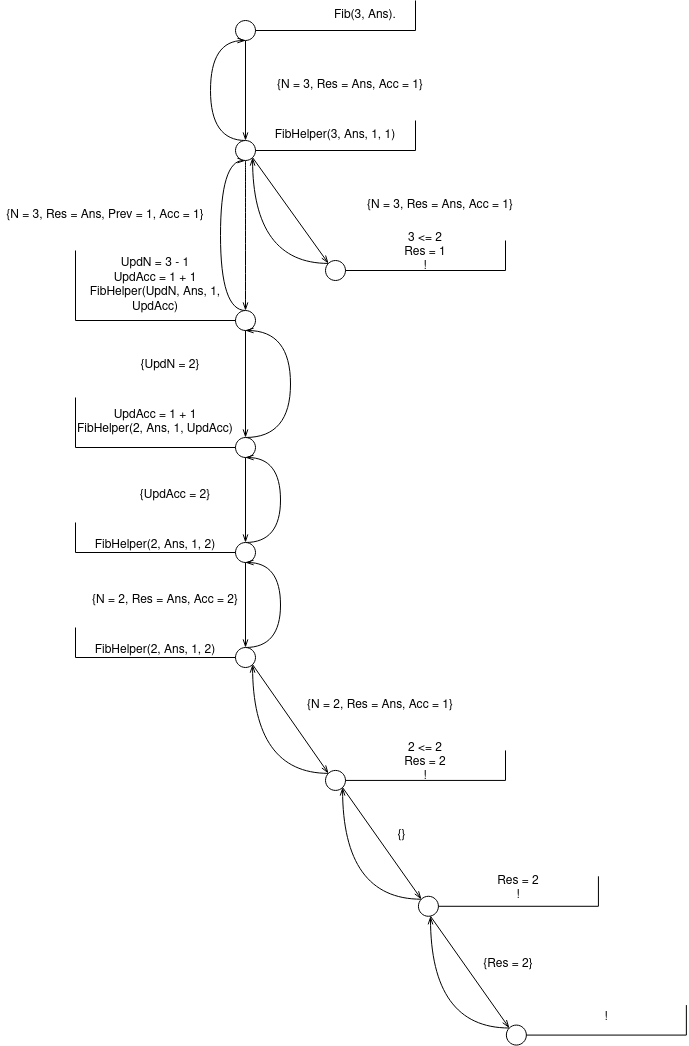
\includegraphics[width=0.75\linewidth]{../additional/tree-cut.drawio.png}
\end{figure}
\begin{figure}[H]
	\centering
	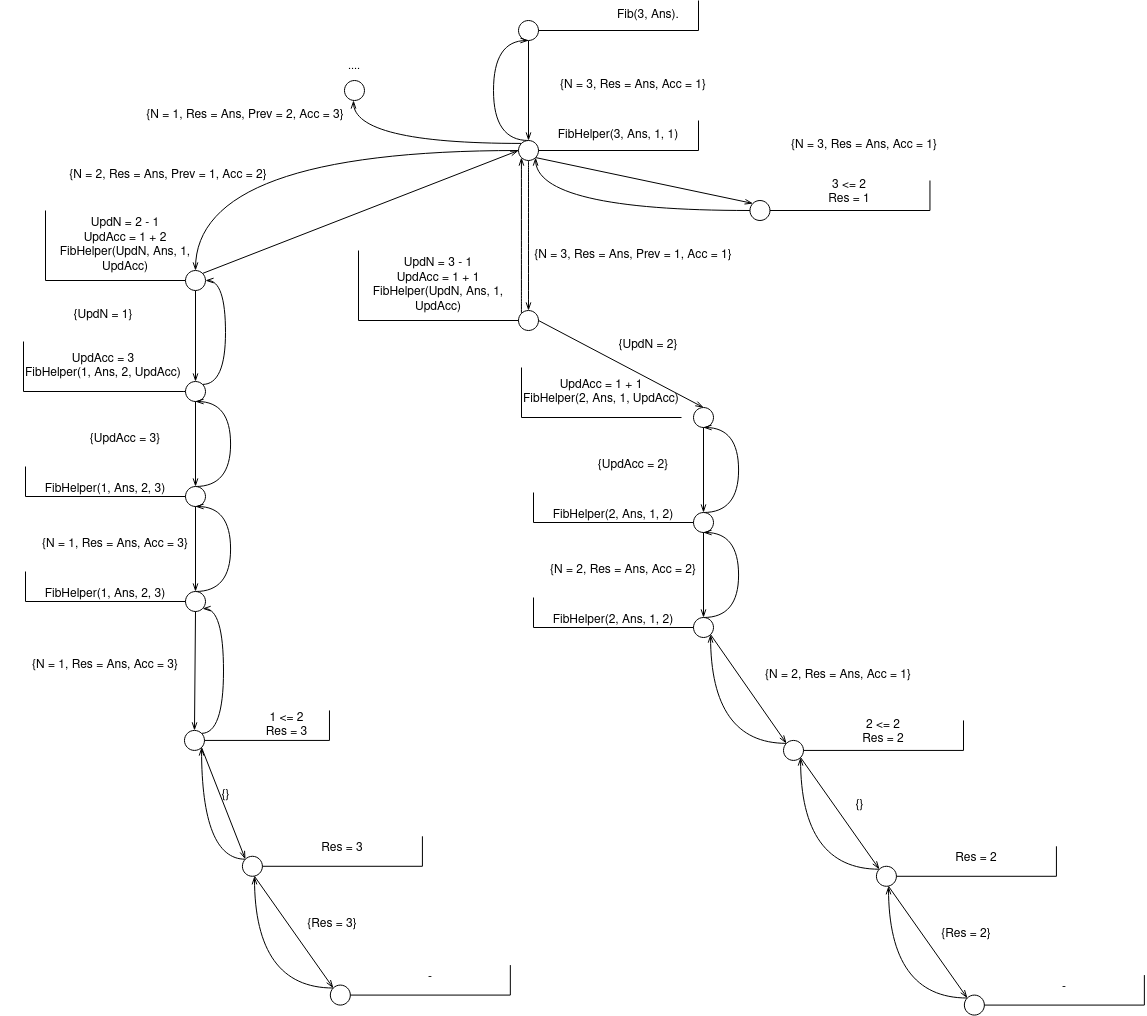
\includegraphics[width=\linewidth]{../additional/tree-no-cut.drawio.png}
\end{figure}
Написать:
\begin{tasks}[label=\arabic*]
	\task Свой reverse;
	\task Программу для нахождения всех списков, которые можно получить из элементов заданного списка.
\end{tasks}

\begin{lstlisting}
all_possible_lists(InList,Out) :- combinations(InList,_,SubList), permutations(SubList,Out).

combinations([], [], []).
combinations([H|T],[H|L],R) :- combinations(T,L,R).
combinations([H|T],L,[H|R]) :- combinations(T,L,R).

permutations([ ],[ ]) :- !.
permutations(L,[X|R]) :- omit(X,L,M), permutations(M,R).

omit(H,[H|T],T).
omit(X,[H|L],[H|R]) :- omit(X,L,R).
\end{lstlisting}

\begin{lstlisting}
reverse([],Z,Z).
reverse([H|T],Z,Acc) :- reverse(T,Z,[H|Acc]).
\end{lstlisting}

Игорк находится в лабиринте MxN клеток. Лабиринт содержит стены и точки телепортации. Найти путь от точки старта до точки финиша. 
\begin{lstlisting}
w(0,0).
w(0,1). w(1,1). w(2,1). w(3,1). w(4,1). w(5,1).
w(1,2).         w(3,2).         w(5,2).
w(1,3).         w(3,3).         w(5,3).
w(0,4). w(1,4). w(2,4).         w(4,4). w(5,4).
w(2,5). w(3,5). w(4,5).

t(w(1, 1), w(3, 3)).
t(w(3, 3), w(5, 3)).

path_exists(X0,Y0,X,Y) :- next_cell(X0,Y0,X,Y), w(X,Y).
next_cell(X0, Y0, X, Y) :- t(w(X0, Y0), w(X_to, Y_to)), X is X_to, Y is Y_to.
next_cell(X0,Y0,X0,Y) :- Y is Y0+1.
next_cell(X0,Y0,X,Y0) :- X is X0+1.
next_cell(X0,Y0,X0,Y) :- Y is Y0-1.
next_cell(X0,Y0,X,Y0) :- X is X0-1.

go(X,Y,X,Y,Path,Path).
go(X0,Y0,X,Y,SoFar,Path) :-
path_exists(X0,Y0,X1,Y1),
\+ memberchk( w(X1,Y1), SoFar),
go(X1,Y1,X,Y,[w(X1,Y1)|SoFar],Path).
\end{lstlisting}